\documentclass{article}
\usepackage{tikz}
\usepackage{amsmath}
\usepackage{amssymb} 
\usepackage[a4paper]{geometry}
\usepackage{fancyhdr}
\pagestyle{fancy}
\lhead{Geraden}
\rhead{März 2025}
\begin{document}
 
\newcommand{\vect}[1]{\overrightarrow{#1}} 
  
\section{Geraden}
\begin{minipage}{\dimexpr\textwidth-6cm}
Eine Gerade beinhaltet alle Punkte, welche in eine bestimmte Richtung zeigen, heißt zu dem Vektor, welcher die Richtung angibt, dem \textbf{Richtungsvektor}, kollinear sind. Ist $\vect{u}$ der Richtungsvektor, entsprechen diese Punkte der Gleichung $r \cdot \vect{u}$ mit $r \in \mathbb{R}$. Damit die Gerade nicht durch den Ursprung gehen muss, werden all diese Punkte um den \textbf{Stützvektor}, oft $\vect{\mathrm{OA}}$, verschoben.
Somit gilt 
\[
 g: \vect{x} = \vect{\mathrm{OA}} + r \cdot \vect{u} 
\] 
Basiert die Gerade auf eine Verbindung von zwei Punkten, kann der Verbindungsvektor dieser als Richtungsvektor verwendet werden. Die Punkte müssen auch im Namen der Gleichung angegeben werden. Wird eine Gerade durch die Punkte $\mathrm{A}$ und $\mathrm{B}$ gelegt, gilt
\end{minipage} 
\hfill
\begin{minipage}{6cm}
  \centering
  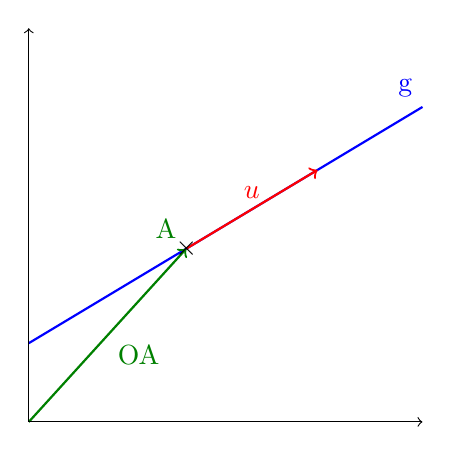
\begin{tikzpicture}
    \draw[thick, blue] (0, 1) -- ++(5, 3) node[above left] {g};
    \draw[->, thick, green!50!black] (0, 0) -- (2, 2.2) node[midway, below right] {$\vect{\mathrm{OA}}$};
    \draw[->, thick, red] (2, 2.2) -- ++(5/3, 1) node[midway, above] {$\vect{u}$}; 
   
    \draw (2, 2.2) node {$\times$} node[green!50!black, above left] {A};
  
    \draw[->] (0, 0) -- (5, 0); 
    \draw[->] (0, 0) -- (0, 5);
  \end{tikzpicture}
\end{minipage}
 
\vspace{1em} 
\[
 g_{\mathrm{AB}}: \vect{x} = \vect{\mathrm{OA}} + r \cdot \vect{\mathrm{AB}} 
\]
 
\subsection{Strecken} 
\begin{minipage}{6cm}
  \centering
  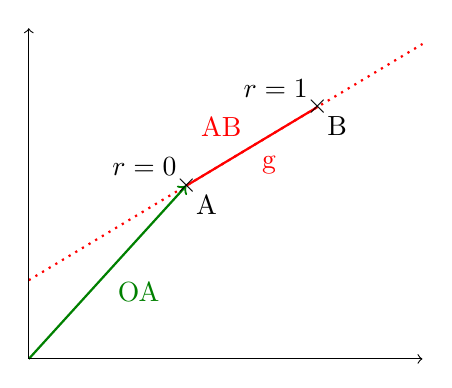
\begin{tikzpicture}
    \draw[dotted, thick, red] (0, 1) -- ++(5, 3);
     
    \draw[->, thick, green!50!black] (0, 0) -- (2, 2.2) node[midway, below right] {$\vect{\mathrm{OA}}$};
    \draw[thick, red] (2, 2.2) -- ++(5/3, 1) node[midway, above left] {$\vect{\mathrm{AB}}$} node[midway, below right] {g};
  
    \draw (2, 2.2) node[black] {$\times$} node[above left] {$r = 0$} node[black, below right] {A};  
    \draw (2+5/3, 3.2) node[black] {$\times$} node[above left] {$r = 1$} node[black, below right] {B};
 
    \draw[->] (0, 0) -- (5, 0); 
    \draw[->] (0, 0) -- (0, 4.2);
  \end{tikzpicture}
\end{minipage}
\hfill 
\begin{minipage}{\dimexpr\textwidth-6cm} 
So wie Strecken nur begrenzte Geraden sind, ist die Parametergleichung einer Strecke auch nur die Parametergleichung einer Gerade auf einem Intervall. Weil für eine Strecke von Punkt $\mathrm{A}$ zu Punkt $\mathrm{B}$ mit der obigen Formel der Endpunkt $\mathrm{A}$ bei $r=0$ liegt (${\vect{\mathrm{OA}} + 0 \cdot \vect{\mathrm{AB}} = \mathrm{A}}$) und bei $r < 0$ die Punkte entgegen der Richtung zu $\mathrm{B}$ gehen würden, von der Strecke herunter, muss $r \geq 0$ sein. Mit der Gleichung Logik für Punkt $\mathrm{B}$, bei $r=1$ ($\vect{\mathrm{OA}} + 1 \cdot \vect{\mathrm{AB}} = \mathrm{B}$), gilt zudem noch $r \leq 1$. Somit gilt insgesamt die generelle Formel 
\[
 g_{\mathrm{AB}}: \vect{x} = \vect{\mathrm{OA}} + r \cdot \vect{\mathrm{AB}}
 \quad \text{mit} \quad
 0 \leq r \leq 1 
\]
\end{minipage} 
 
\subsection{Spurpunkte}
Spurpunkte sind die Schnittpunkte einer Gerade mit den Koordinatenebenen.
Eine dreidimensionale Gerade kann bis zu drei Spurpunkte haben, eine für jede Dimension. Die Schnittpunkt werden nach den Koordinaten, welche nicht null sind, benannt. \newline
Ein Schnittpunkt mit der Ebene $x_2x_3$ liegt bei $x_1 = 0$, heißt der Schnittpunkt ist
\[
 S_{23} = \begin{pmatrix} 0 \\ x_2 \\ x_3 \end{pmatrix} 
\]
Dieser Vektor kann mit der Parametergleichung gleichgesetzt werden um das fehlende $r$ und die fehlenden Koordinaten, in diesem Fall $x_2$ und $x_3$, zu bestimmen. Wenn es keine Lösung gibt, gibt es keinen Spurpunkt, weil die Gerade nicht durch die Ebene geht.
 

\end{document}
 
 
 
 
 
 
 
